\documentclass{beamer}
\usepackage{lipsum}
\usepackage[brazilian]{babel}
\usepackage[utf8]{inputenc}

\usepackage{enumerate}
\usepackage{dcolumn}
\usepackage{tabu}
\usepackage{colortbl}
\usepackage{booktabs}
\usepackage{changes}
\usepackage{listings}
\usepackage{placeins}
\usepackage{amsmath}

\usepackage{multirow}

\newcommand*{\Scale}[2][4]{\scalebox{#1}{$#2$}}%
\newcommand*{\Resize}[2]{\resizebox{#1}{!}{$#2$}}%

\usetheme[faculty=ppca,language=logo,framenumber,totalframenumber]{UniversiteitGent}

\title{ERLANGMS: Implantação de um barramento de serviços no CPD/UnB}
\subtitle{ \textcolor{forestgreen}{Universidade de Brasília} \\
			\textcolor{black}{Centro de Informática} \\
			3 de Maio de 2017
}
\author{Everton de Vargas Agilar \\
		E-mail: evertonagilar@unb.br
}



\begin{document}

\begin{frame}
  \titlepage
\end{frame}




%%##############################################################




\subsection{Plan}

\begin{frame}
  \frametitle{Plano}

    \begin{itemize}
  	  \item<1-> Contexto
   	  \item<1-> Objetivos
    	  \item<1-> Justificativa
  	  \item<1-> Research Questions
  	  \item<1-> Search Strategy
  	  \item<1-> Results
   	  \item<1-> Conclusions/Future Works
    \end{itemize}

\end{frame}




%%##############################################################




\section{Introdução}


\subsection{Contexto}


\begin{frame}
  \frametitle{Contexto}

  \begin{exampleblock}{Modernização de Sistemas Legados}
  
  “\textbf{Legacy information systems} are typically the
	backbone of an organization’s information flow
	and the main vehicle for consolidating business
	information. They are thus mission critical, and
	their failure can have a serious impact on
	business.” [BENNET95]

	\vspace{0.5cm} 

	“Migrate Systems Incrementally recommends that the old system be
	gradually and incrementally replaced by the new system. New
	results can then be integrated as you proceed...” [DEMEYER et al. 2002]
  \end{exampleblock}

  
\end{frame}




%%##############################################################




\subsection{Contexto}


\begin{frame}
  \frametitle{Contexto}

  \begin{exampleblock}{Relatório de Gestão do CPD/UnB 2010-2012}
  
		“Foi identificada a necessidade de remodelação de todos os sistemas
da UnB visando uma atualização tecnológica e uma melhor
integração de seus fluxos.” ... [cpd.unb.br/transparencia]

    \begin{itemize}
  	  \item<1-> Alto custo de manutenção para manter os sistemas legados;
   	  \item<1-> Duplicação das regras de negócio entre os sistemas;
  	  \item<1-> Dificuldades para integrar os sistemas.
    \end{itemize}


  \end{exampleblock}

  
\end{frame}




%%##############################################################






%%##############################################################




\subsection{Objetivos}


\begin{frame}
  \frametitle{Objetivos}
  
    \begin{itemize}
       \item<1-> Propor uma abordagem para modernizar os sistemas legados de
forma orientada a serviços (SOA) composto por:

    \begin{itemize}
       \item<1->barramento de serviços próprio desenvolvido em Erlang/OTP;
       \item<1->processo de modernização para guiar os trabalhos de modernização 
       e disponibilizar uma arquitetura de software padronizada;
       \item<1->kit de desenvolvimento (SDK) para implementar serviços independente da
       linguagem de programação.
    \end{itemize}
				
    \end{itemize}
    
\end{frame}



%%##############################################################



\subsection{Justificativa}


\begin{frame}
  \frametitle{Justificativa}
  
    \begin{itemize}
       \item<1-> Permitir maior reuso dos fluxos de negócios e maximização da
modularidade das aplicações;
       \item<1-> Experimentar SOA (Service Oriented Architecture);
       \item<1-> Obter uma arquitetura documentada e padronizada para modernização de software.

				
    \end{itemize}
    
\end{frame}




%%##############################################################




\section{Results}


\subsection{Research Questions}


\begin{frame}
  \frametitle{Research Questions}

  \begin{exampleblock}{Research Questions}
  
	  \begin{itemize}
	    \item<1->(QP1) What characterizes the modernization of legacy 
	    				  systems according to the existing literature?
    	\item<2->(QP2) What processes, techniques, and tools have been
				   suggested in the literature to support modernization
				   activities of legacy systems?
		\item<3->(QP3) What are the reasons that lead organizations to 
					  modernize their legacy systems?
	  \end{itemize}
  
  \end{exampleblock}

  
\end{frame}



%%##############################################################



\subsection{Search Strategy}


\begin{frame}
  \frametitle{Search Strategy}

  	\begin{itemize}
	    \item<1->Analyzed 44 publications in major
				conferences and journals Engineering area
				Software (CMRS, ICSE, ICSM, among others);
	    \item<2->The search strategy consists of a manual search 
	    			activity for articles complemented 
	    			by technical "snowball";
		\item<3->Selected publications between 1995 and 2015.
	\end{itemize}
  
  	%% Mostra o esquema do protocolo de pesquisa
  	
	\begin{figure}
	\centering
		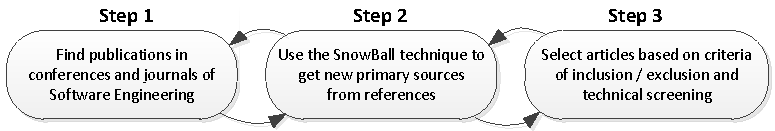
\includegraphics[scale=0.6]{img/protocolo_pesquisa_ms.pdf}
		\caption{Scheme of the research protocol.}
	\end{figure}
  
\end{frame}





%%##############################################################



\subsection{View of the studies identified}


\begin{frame}
  \frametitle{View of the studies identified}

 	%% Mostra o diagrama de bolhas
  	
	\begin{figure}
	\centering
		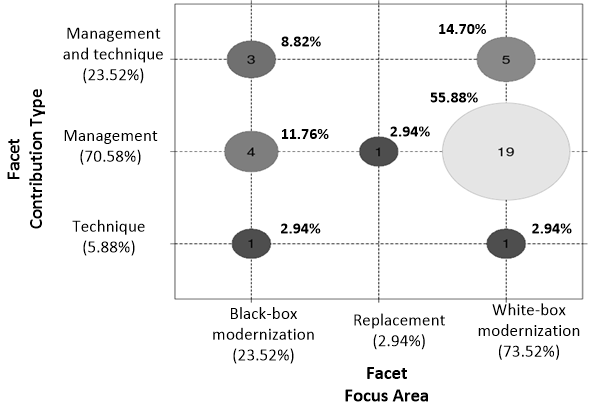
\includegraphics[scale=0.5]{img/bubble_diagram.png}
	\end{figure}
  
\end{frame}




%%##############################################################



\subsection{Terms most frequently cited in selected publications}



\begin{frame}
  \frametitle{Terms most frequently cited in selected publications}

 	%% Mostra o diagrama de bolhas
  	
	\begin{figure}
		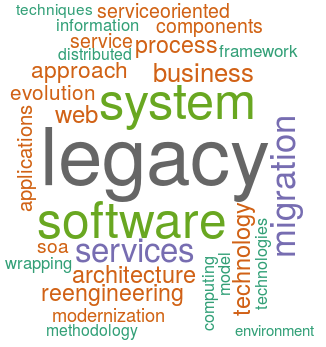
\includegraphics[scale=0.4]{img/word_cloud.png}
	\end{figure}

\end{frame}




%%##############################################################



\section{Conclusions and Future Work}


\subsection{Conclusions and Future Work}


\begin{frame}
  \frametitle{Conclusions and Future Work}

  \begin{itemize}
    \item<1->We have presented the results of a mapping study (MS) that 
    			consolidates the main contributions to the field;
    \item<1->We found that the majority of the publications 
    			relies on a kind white-box modernization 
    			approach;
	\item<1->We also find that the managerial aspects are most 
			relevant, which reinforces the idea of a good
			strategy of modernization;
	\item<1->However, we found just a few studies reporting success 
			experiences in modernizing legacy systems;
	\item<1->As future work, we planned a service-oriented approach to 
			modernizing legacy systems of UnB.
  \end{itemize}
  
\end{frame}




%%##############################################################


\subsection{Questions}

%% Principais Desafios do CPD/UnB

\begin{frame}[c]{ }
\centering
  \huge{Questions and remarks ?}
\end{frame}



\end{document}



